\documentclass[tikz,border=10pt]{standalone}
\usepackage{amsmath}
\usepackage{tikz}
\usetikzlibrary{arrows.meta,calc,positioning}

\tikzset{
  signal/.style={->, line width=1.2pt, draw=black!80, >=Stealth},
  block/.style={draw=blue!70!black, line width=1.2pt, rectangle, minimum width=2.0cm, minimum height=1.0cm, fill=none},
  sum/.style={
    draw=green!55!black, line width=1.2pt, circle, minimum size=0.56cm, inner sep=0pt, fill=none,
    path picture={
      \draw[green!55!black, line width=0.9pt]
        (path picture bounding box.south west) -- (path picture bounding box.north east)
        (path picture bounding box.north west) -- (path picture bounding box.south east);
    }
  },
  tap/.style={draw=orange!85!black, line width=1.2pt, circle, minimum size=4.5pt, inner sep=0pt, fill=none},
  small/.style={font=\small}
}

\begin{document}
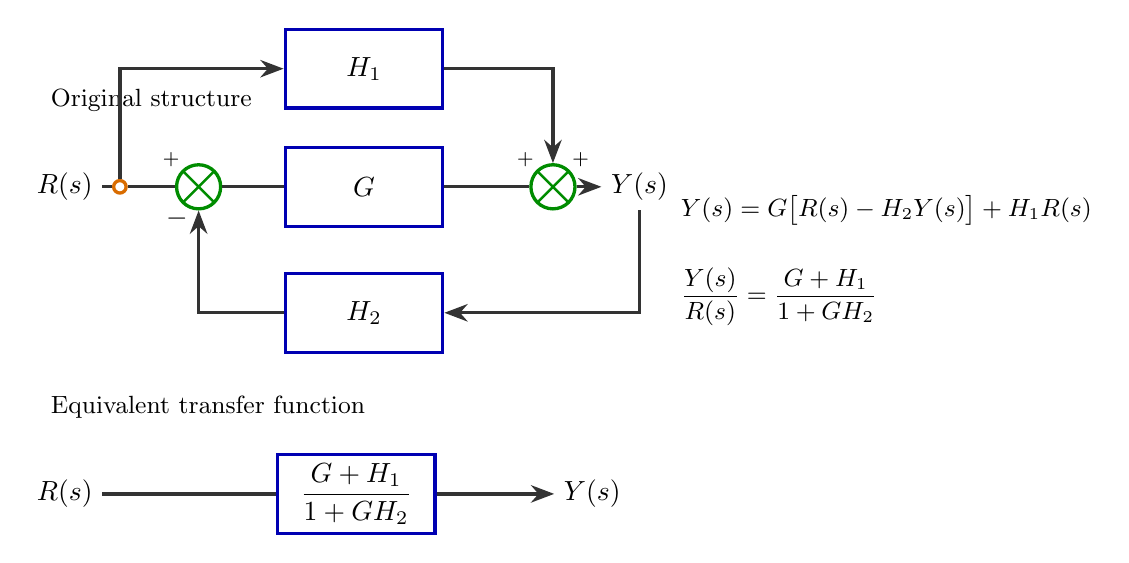
\begin{tikzpicture}
  \node[small, anchor=west] at (0,3.8) {Original structure};
  \node (r) at (0.3,2.7) {$R(s)$};
  \node[tap] (tp) at (1.0,2.7) {};
  \node[sum] (s1) at (2.0,2.7) {};
  \node[block] (g) at (4.1,2.7) {$G$};
  \node[sum] (s2) at (6.5,2.7) {};
  \node (y) at (7.6,2.7) {$Y(s)$};
  \node[block] (h1) at (4.1,4.2) {$H_1$};
  \node[block] (h2) at (4.1,1.1) {$H_2$};

  \draw[signal] (r) -- (tp) -- (s1) -- (g) -- (s2) -- (y);
  \draw[signal] (tp) |- (h1);
  \draw[signal] (h1) -| (s2);
  \draw[signal] (y) |- (h2);
  \draw[signal] (h2) -| node[pos=0.96, left] {$-$} (s1.south);
  \node[font=\scriptsize] at ($(s1)+(-0.35,0.35)$) {$+$};
  \node[font=\scriptsize] at ($(s2)+(-0.35,0.35)$) {$+$};
  \node[font=\scriptsize] at ($(s2)+(0.35,0.35)$) {$+$};

  \node[small, anchor=west] at (0,-0.1) {Equivalent transfer function};
  \node (r2) at (0.3,-1.2) {$R(s)$};
  \node[block] (eq) at (4.0,-1.2) {$\dfrac{G+H_1}{1+GH_2}$};
  \node (y2) at (7.0,-1.2) {$Y(s)$};
  \draw[signal] (r2) -- (eq) -- (y2);

  \node[small, anchor=west] at (8.0,2.4) {$Y(s)=G\bigl[R(s)-H_2Y(s)\bigr]+H_1R(s)$};
  \node[small, anchor=west] at (8.0,1.3) {$\dfrac{Y(s)}{R(s)}=\dfrac{G+H_1}{1+GH_2}$};
\end{tikzpicture}
\end{document}
